\begin{figure}[!htbp] \centering
\subsection{BDD Hardware}
{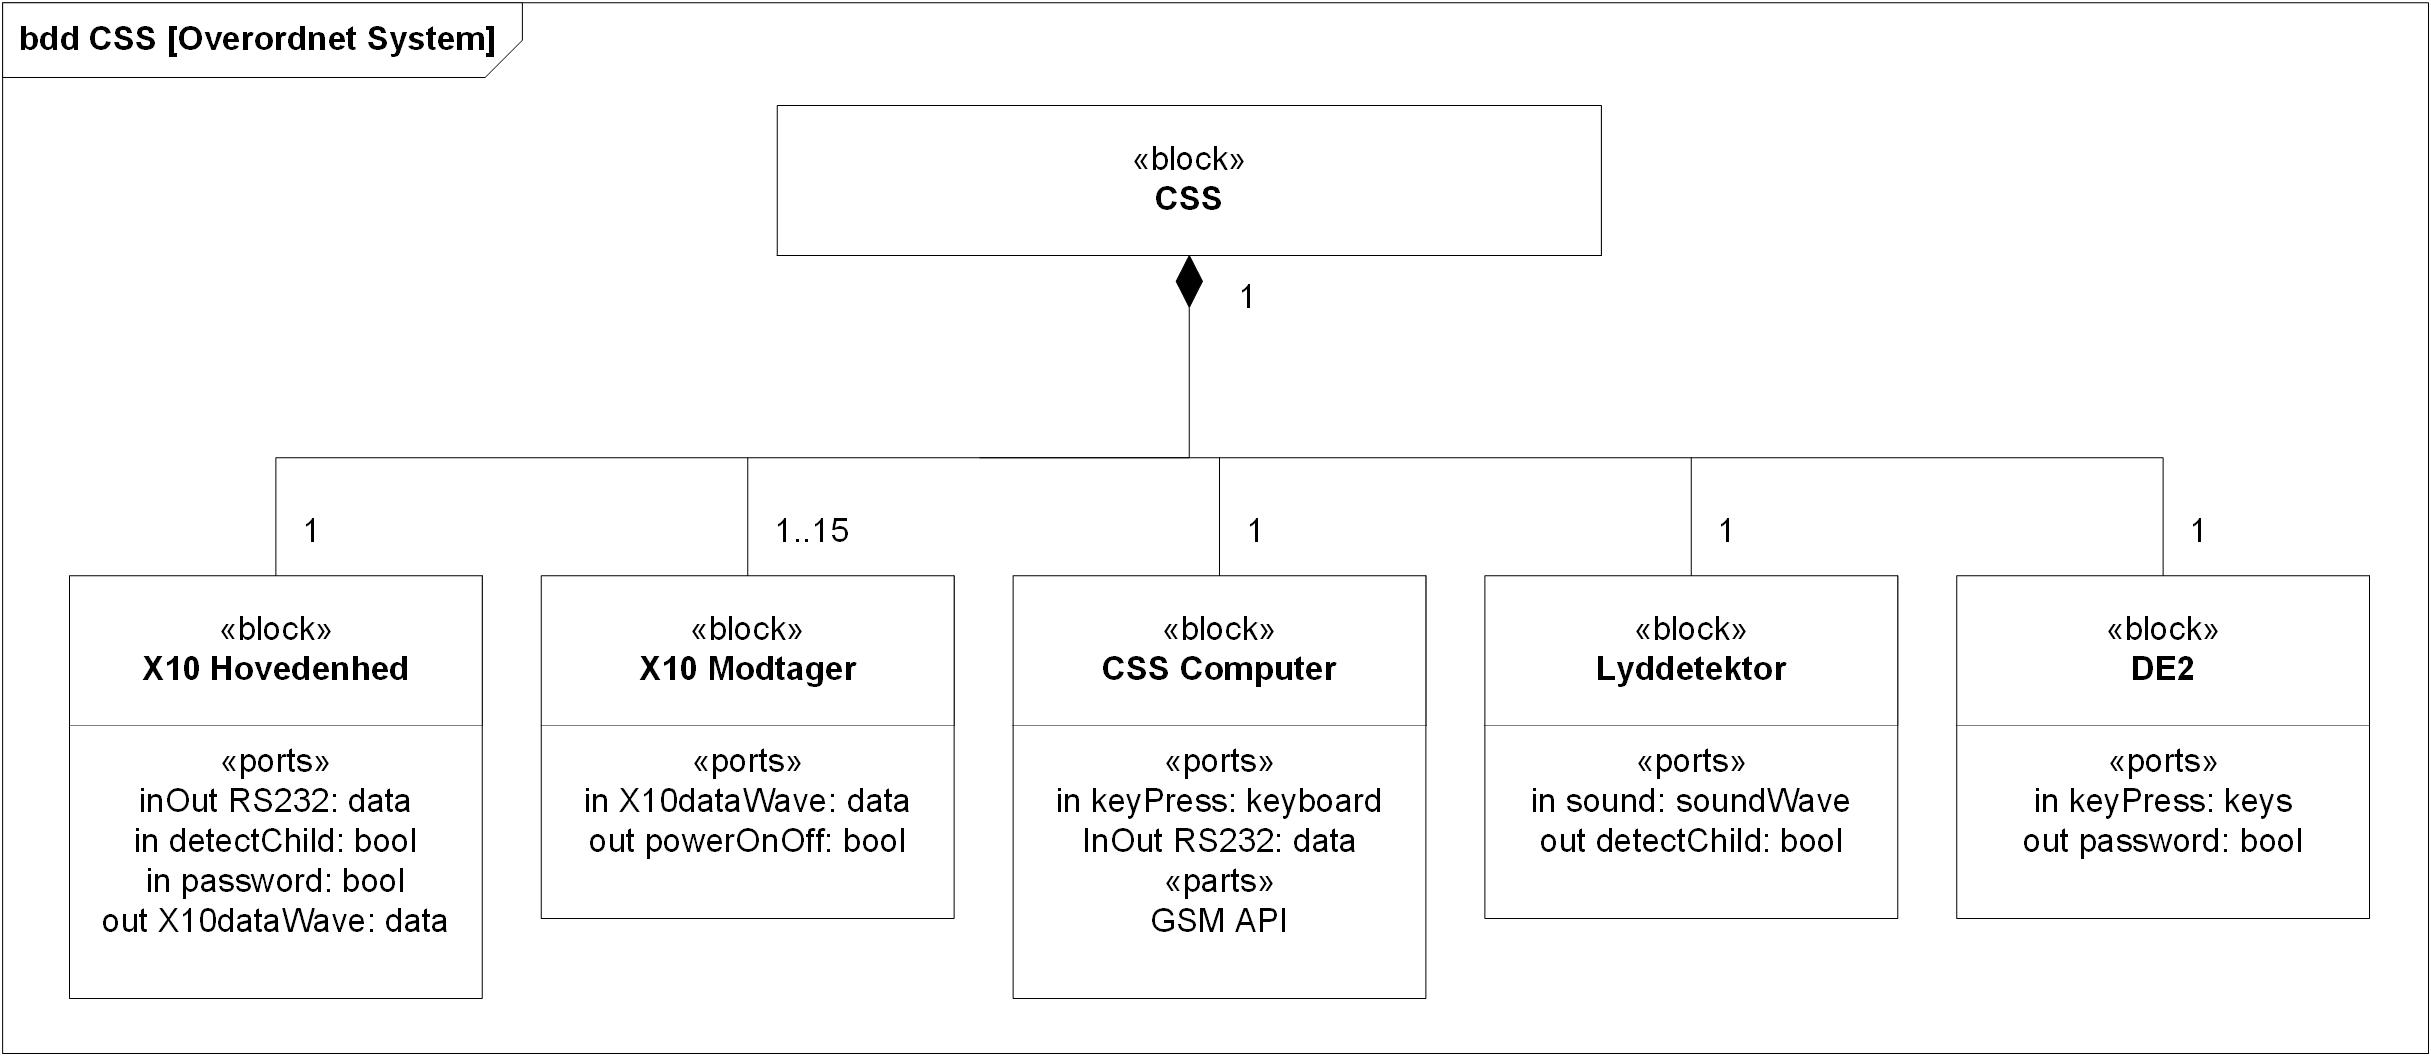
\includegraphics[width=0.9\textwidth]{billeder/diagrammer/BDD_Hardware}}
\caption{BDD Hardware}
\label{lab:bddhardware}
\raggedright
\end{figure}
BDD diagrammet giver et overblik over hvad det samlede system består af. Vi ser en portbeskrivelse som viser hvilke signaler hver blok består af.

\begin{figure}[!htbp] \centering
\subsection{BDD Hovedenhed}
{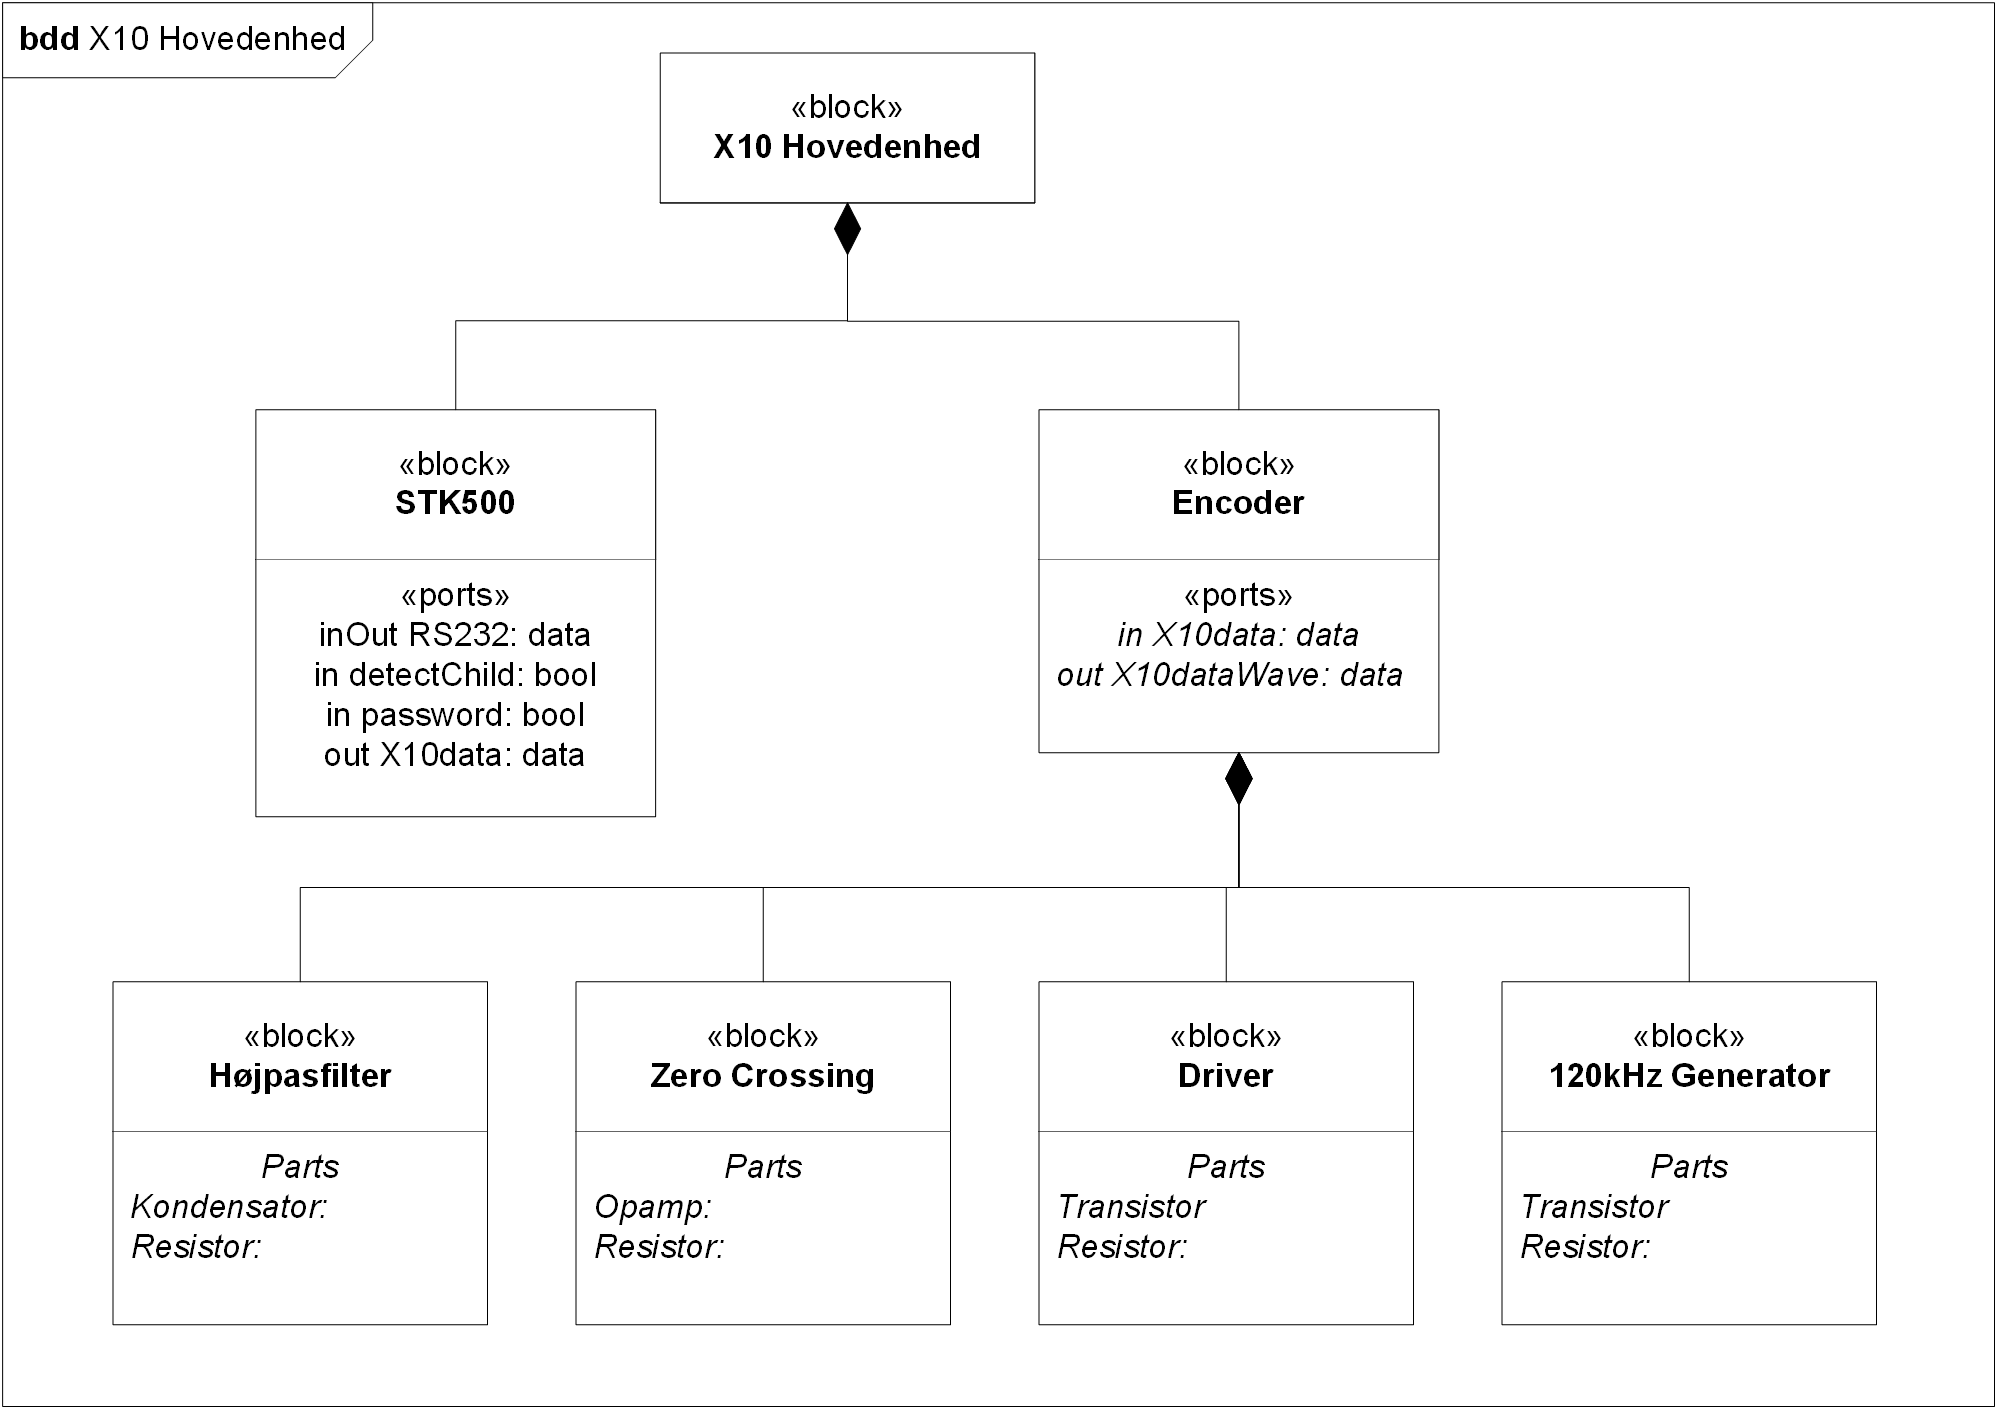
\includegraphics[width=0.9\textwidth]{billeder/diagrammer/BDD_Hovedenhed}}
\caption{BDD Hovedenhed}
\label{lab:bddhovedenhed}
\raggedright
\end{figure}
BDD diagrammet giver et overblik over hvad CSS-hovedenheden består af. Vi ser en portbeskrivelse for STK-kittet og encoder. 

\begin{figure}[!htbp] \centering
\subsection{BDD X10-udtag}
{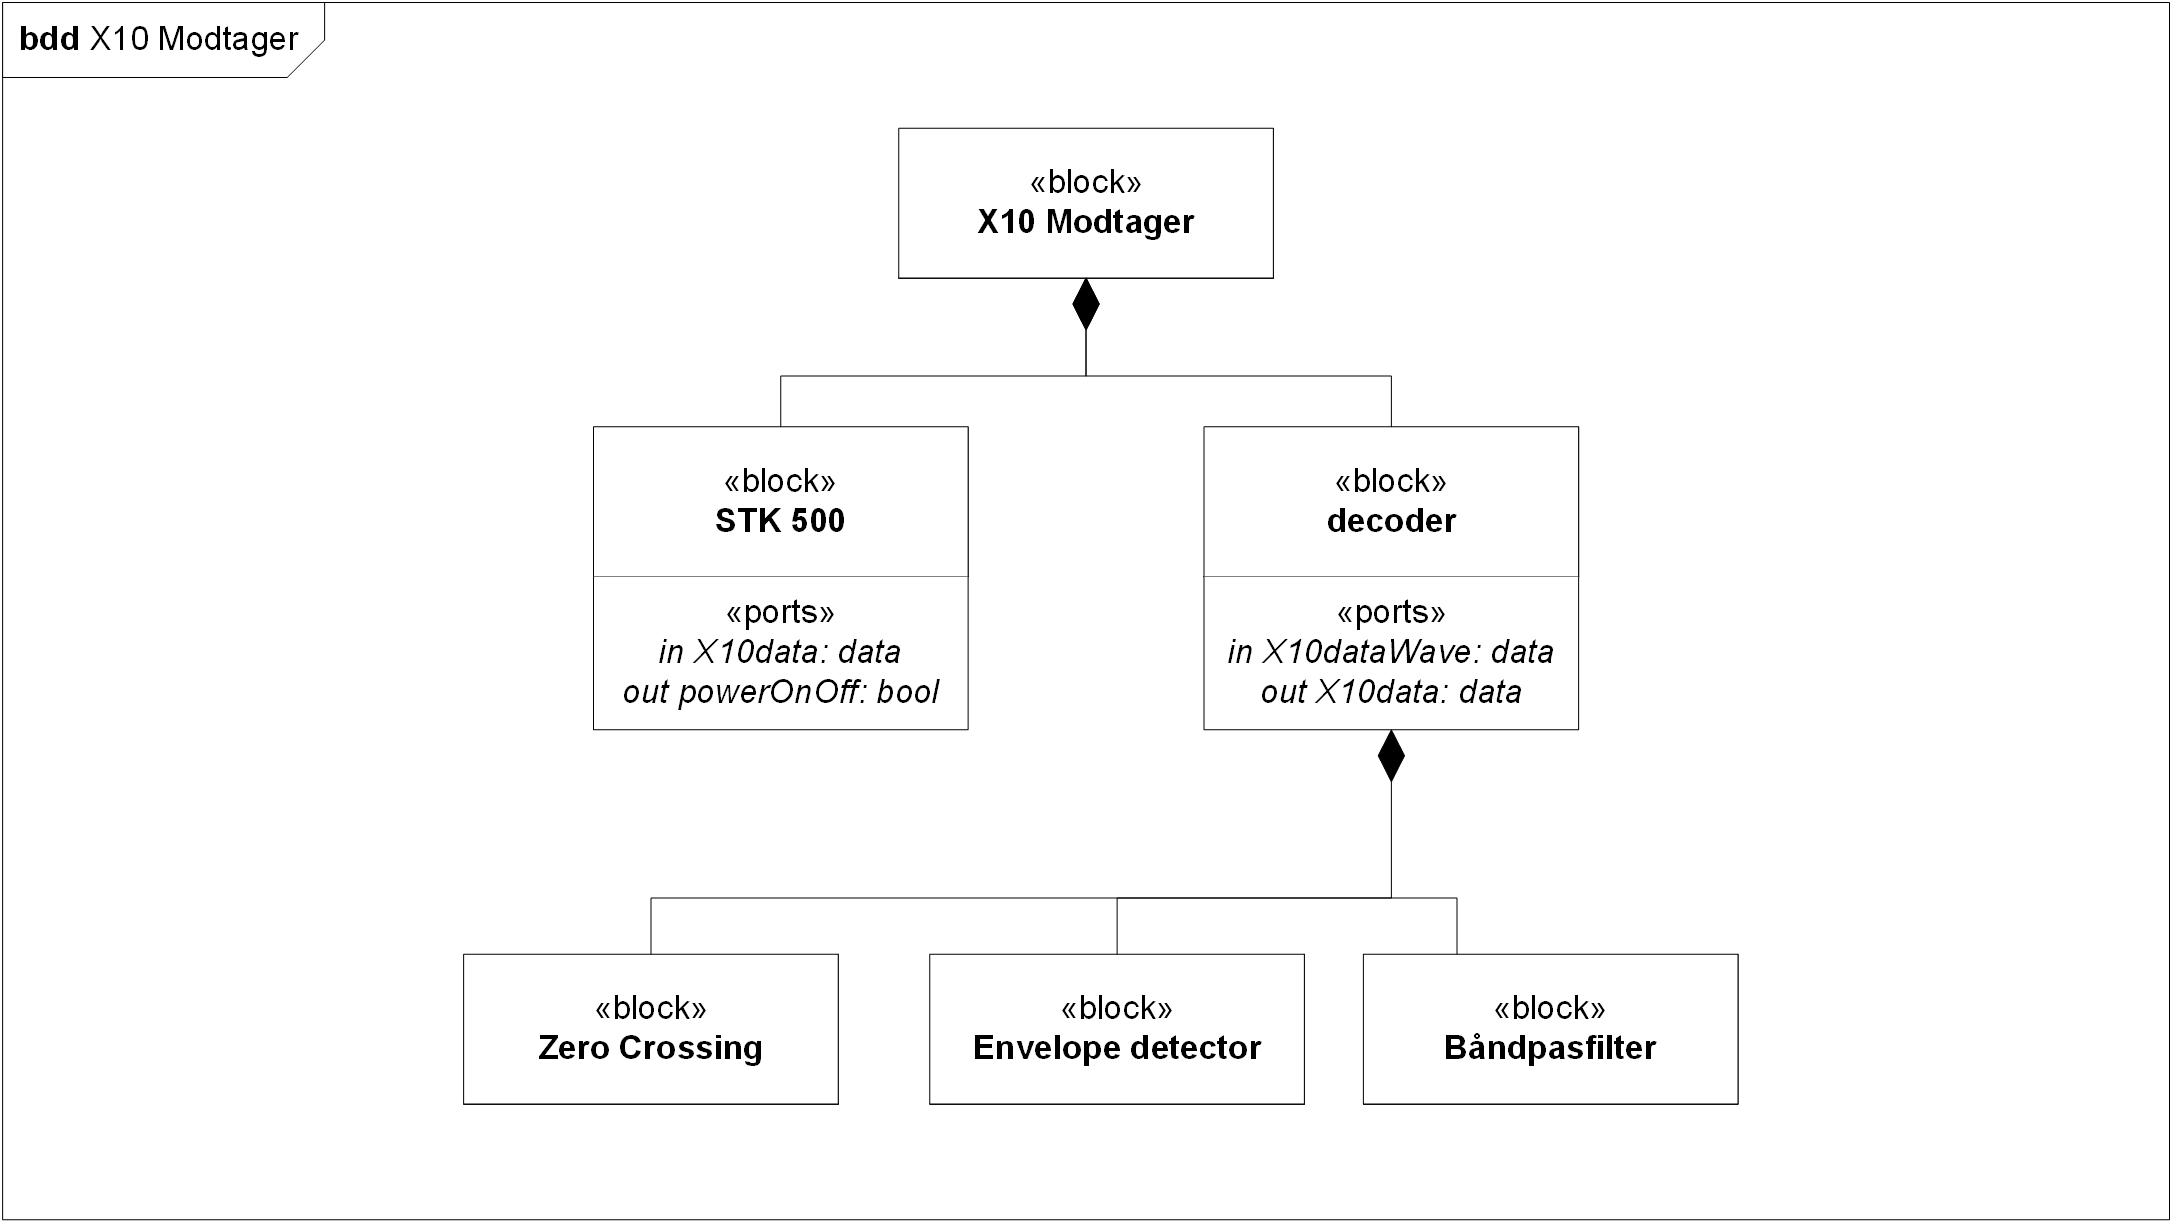
\includegraphics[width=0.9\textwidth]{billeder/diagrammer/BDD_Modtager}}
\caption{BDD X10-udtag}
\label{lab:bddmodtager}
\raggedright
\end{figure}
BDD diagrammet giver et overblik over hvad X10-udtaget består af. Vi ser en portbeskrivelse for STK-kittet og decoderen.

\begin{figure}[!htbp] \centering
\subsection{Plantegning over HW}
{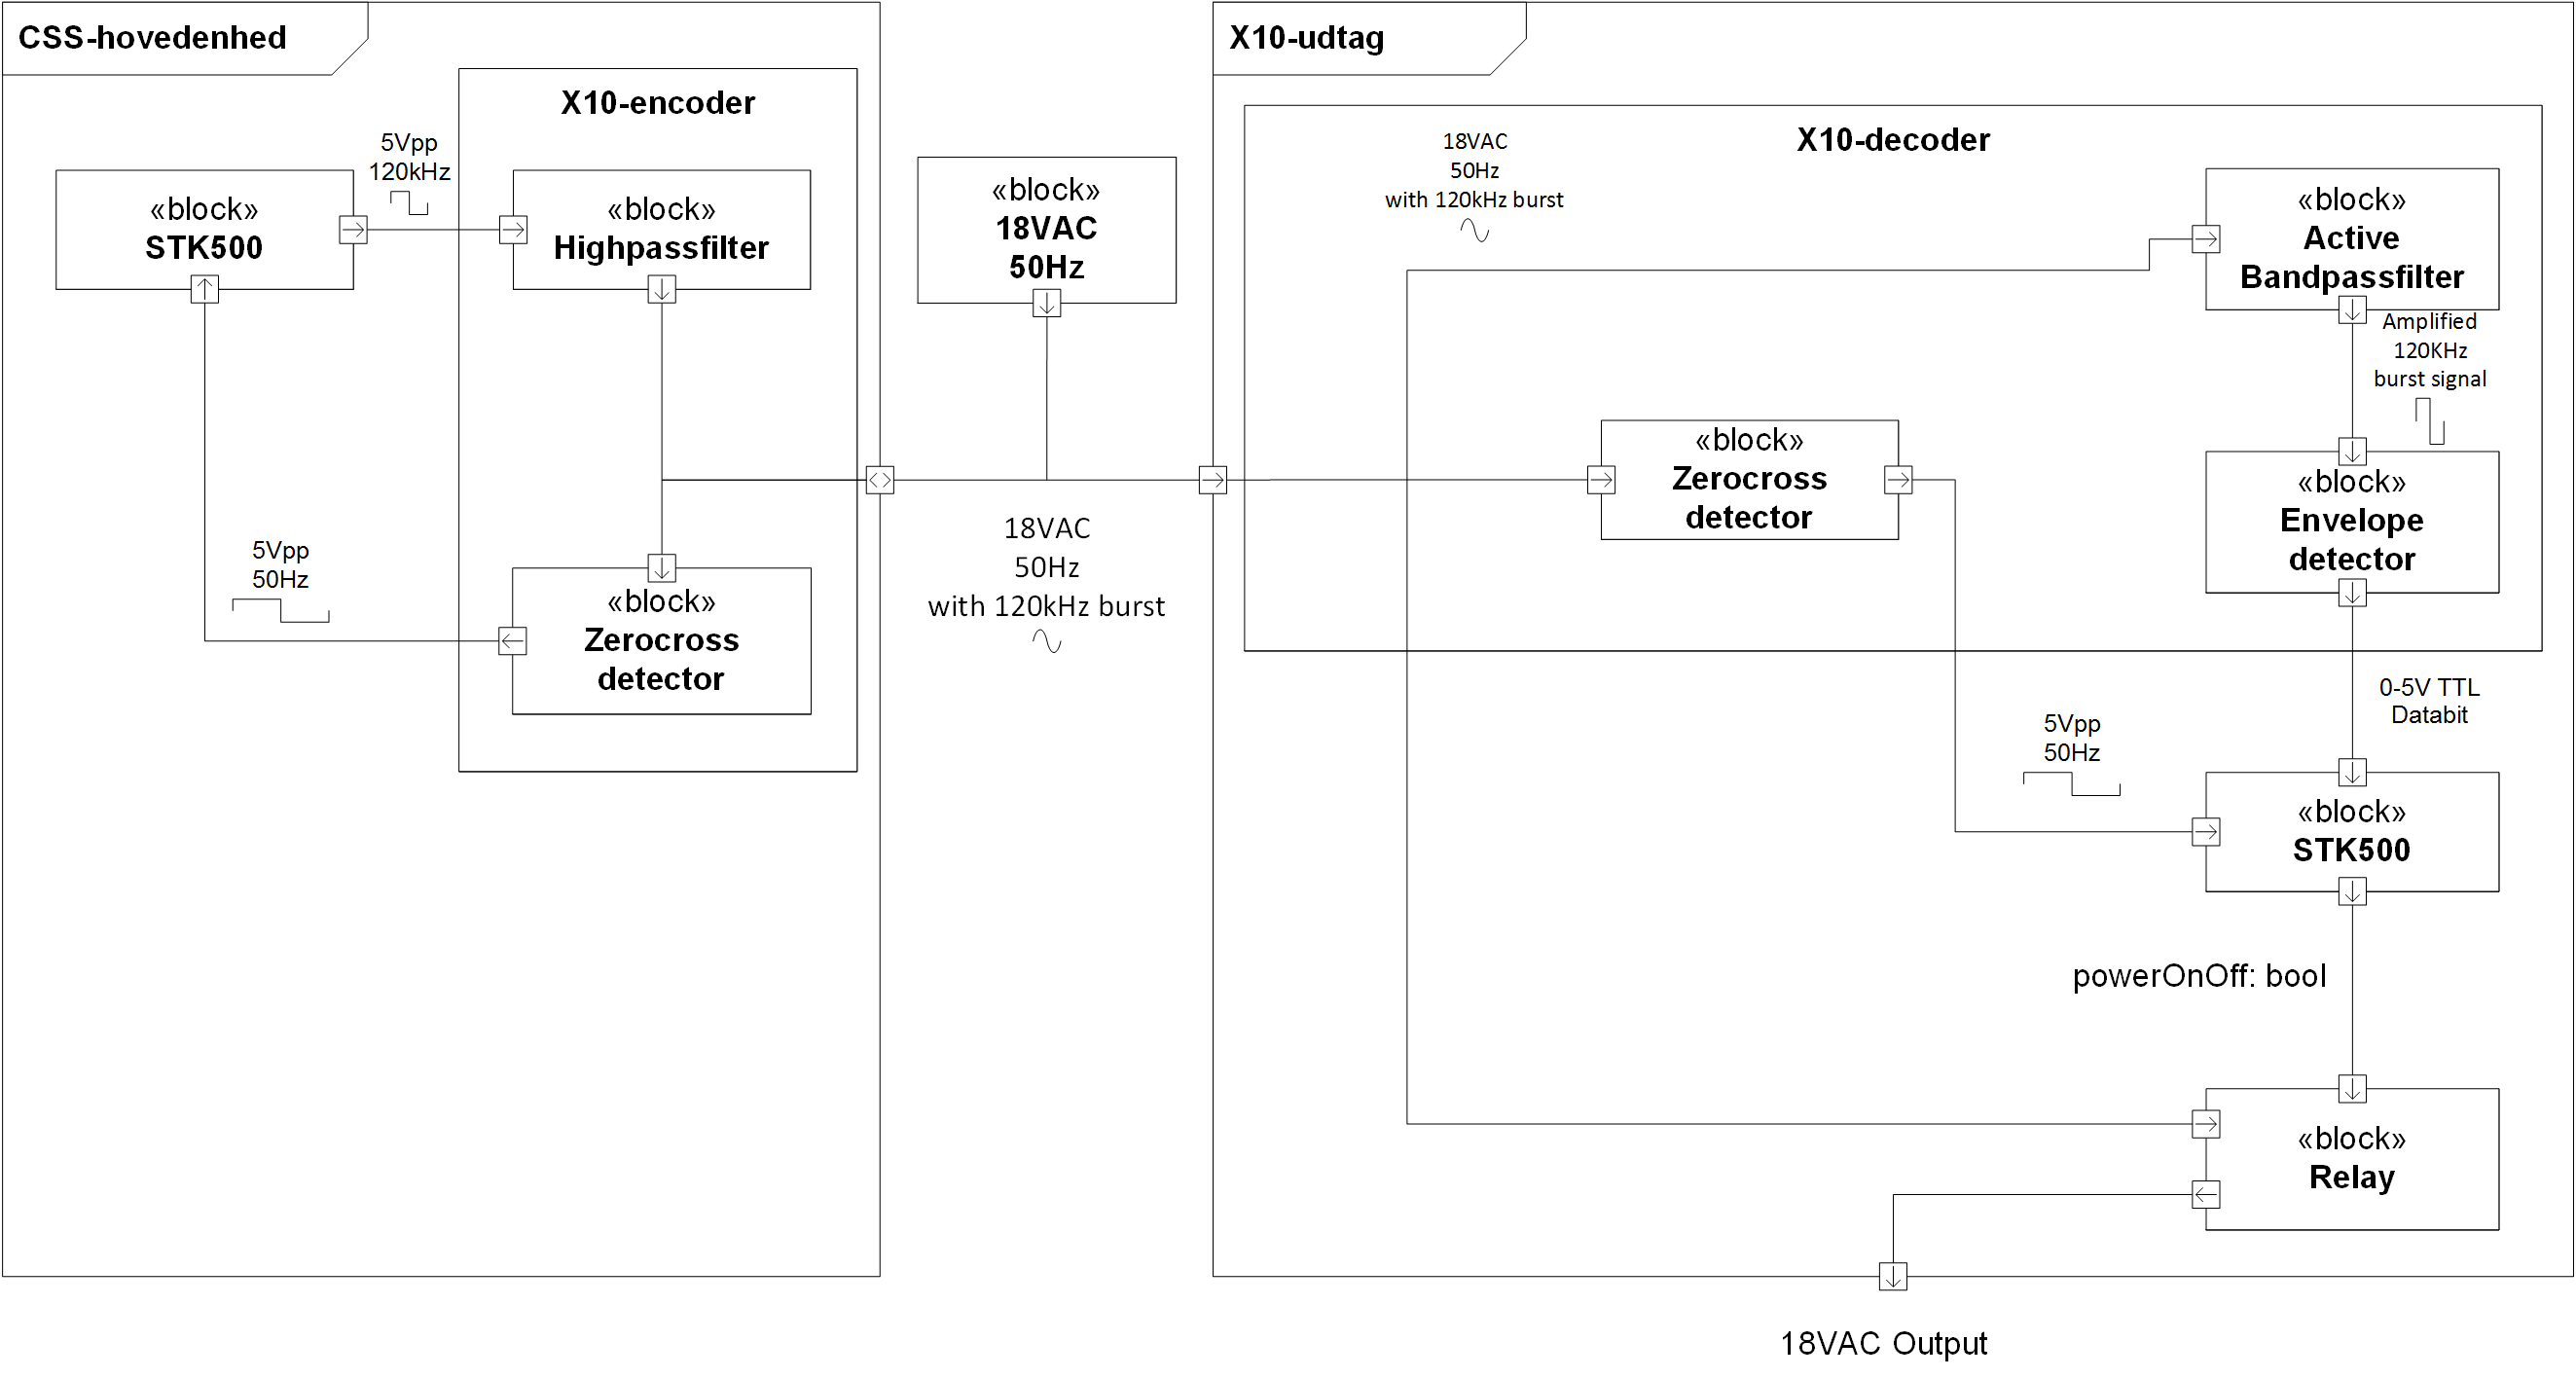
\includegraphics[width=0.9\textwidth]{billeder/diagrammer/Plantegning_over_HW}}
\caption{Plantegning over HW}
\label{lab:Plantegning over HW}
\raggedright
\end{figure}
Plantegningen over hardwaren giver et overblik over hvordan CSS-hovedenheden og X10-udtaget er forbundet, samt hvilke type signaler der bliver sendt imellem dem.

\begin{figure}[!htbp] \centering
\subsection{IBD Hardware}
{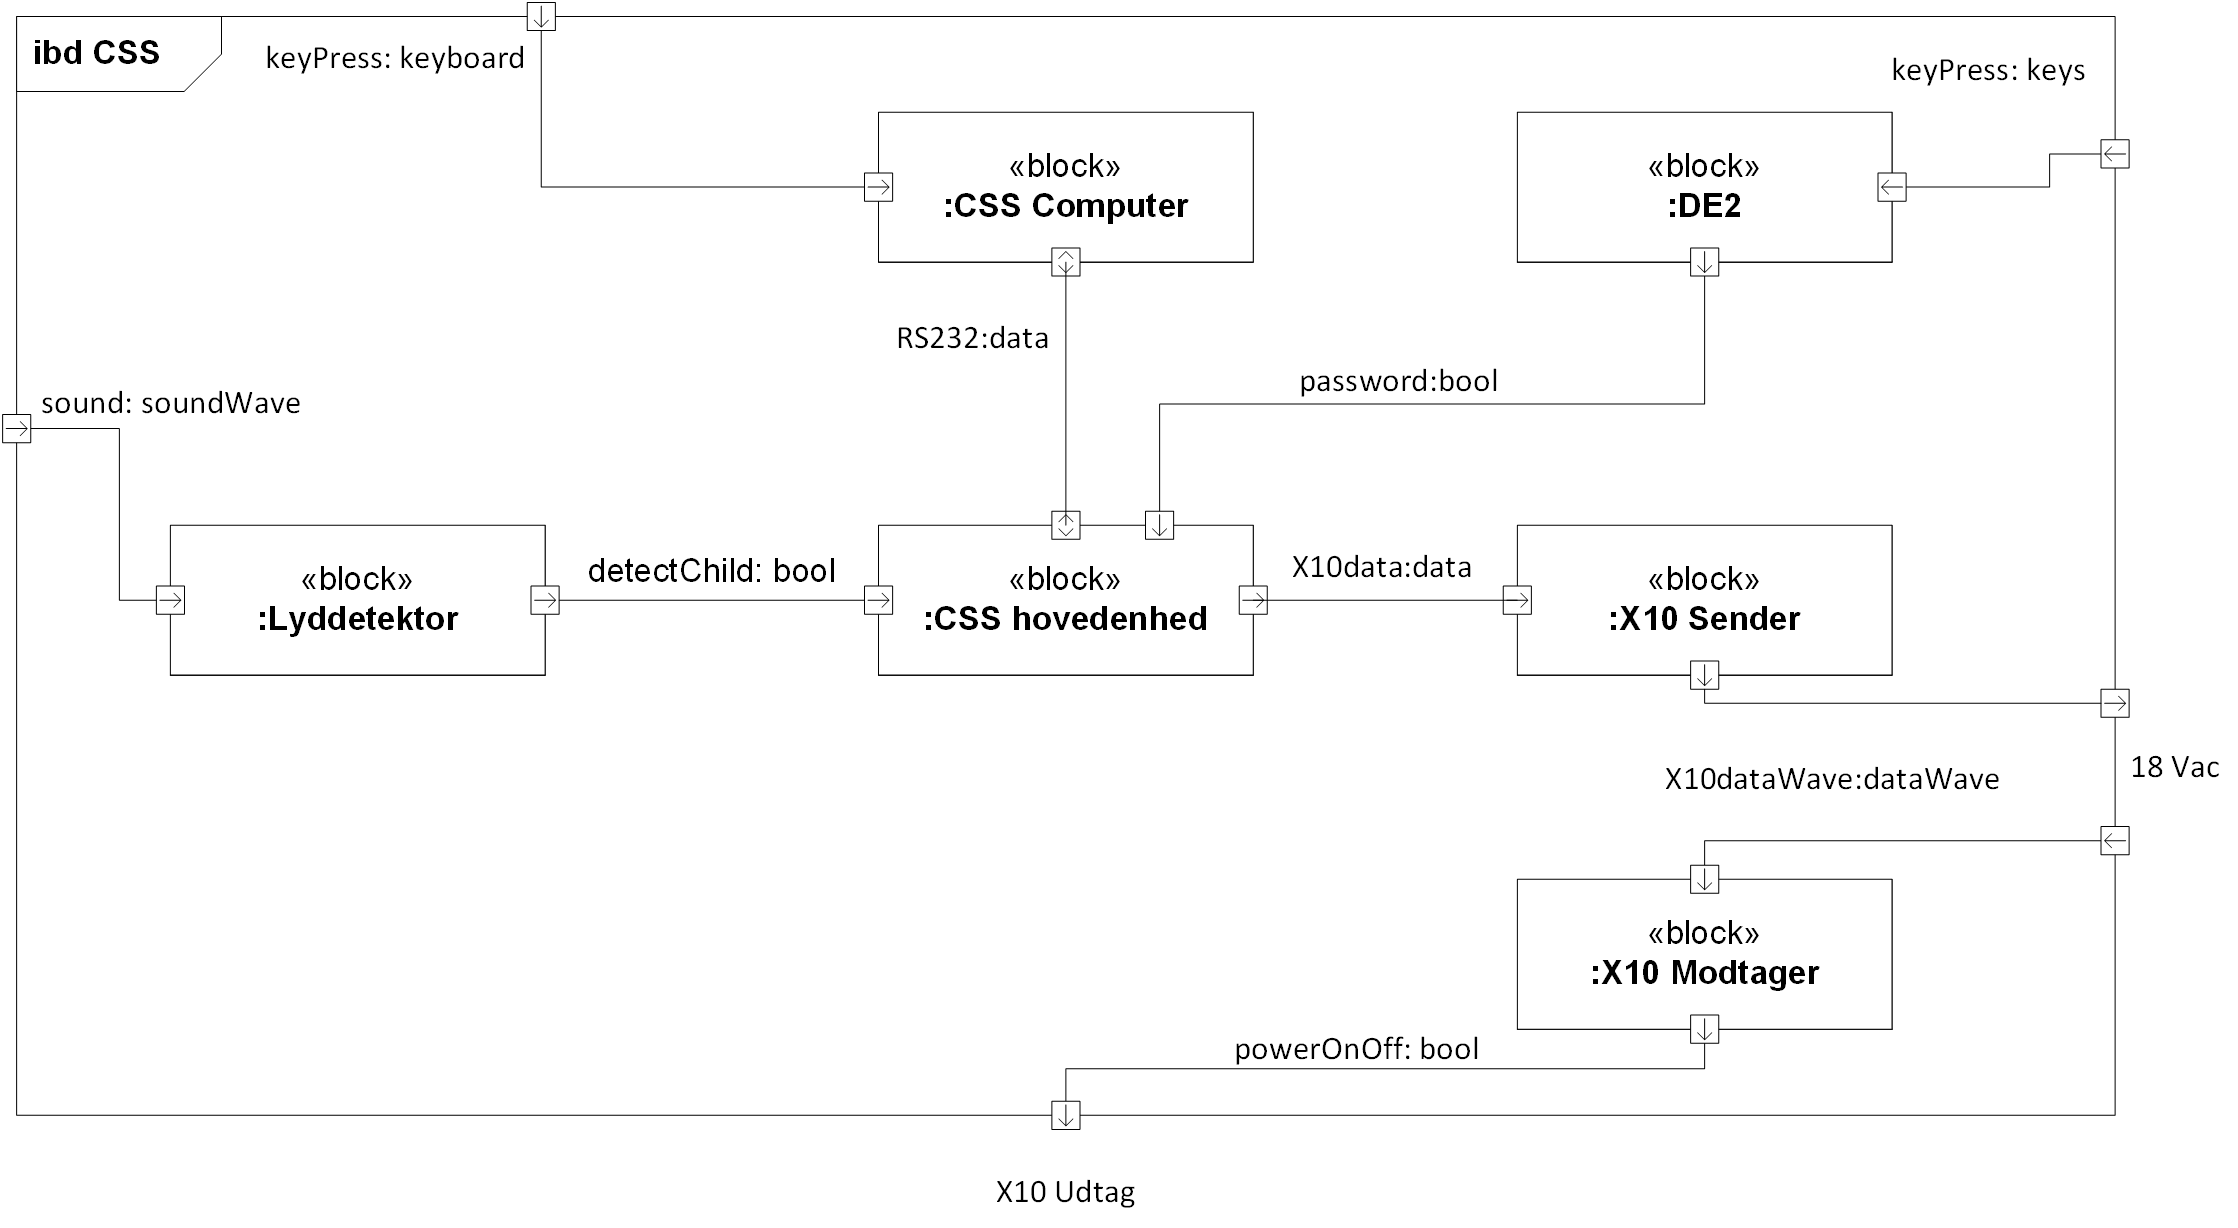
\includegraphics[width=0.9\textwidth]{billeder/diagrammer/IBD_Hardware}}
\caption{IBD Hardware}
\label{lab:ibdhardware}
\raggedright
\end{figure}
IBD diagrammet giver et internt overblik over hvordan hele vores system er forbundet. Vi ser hvilke type signaler der bliver sendt imellem de forskellige blokke.

\begin{figure}[!htbp] \centering
\subsection{IBD CSS-hovedenhed og X10-udtag}
{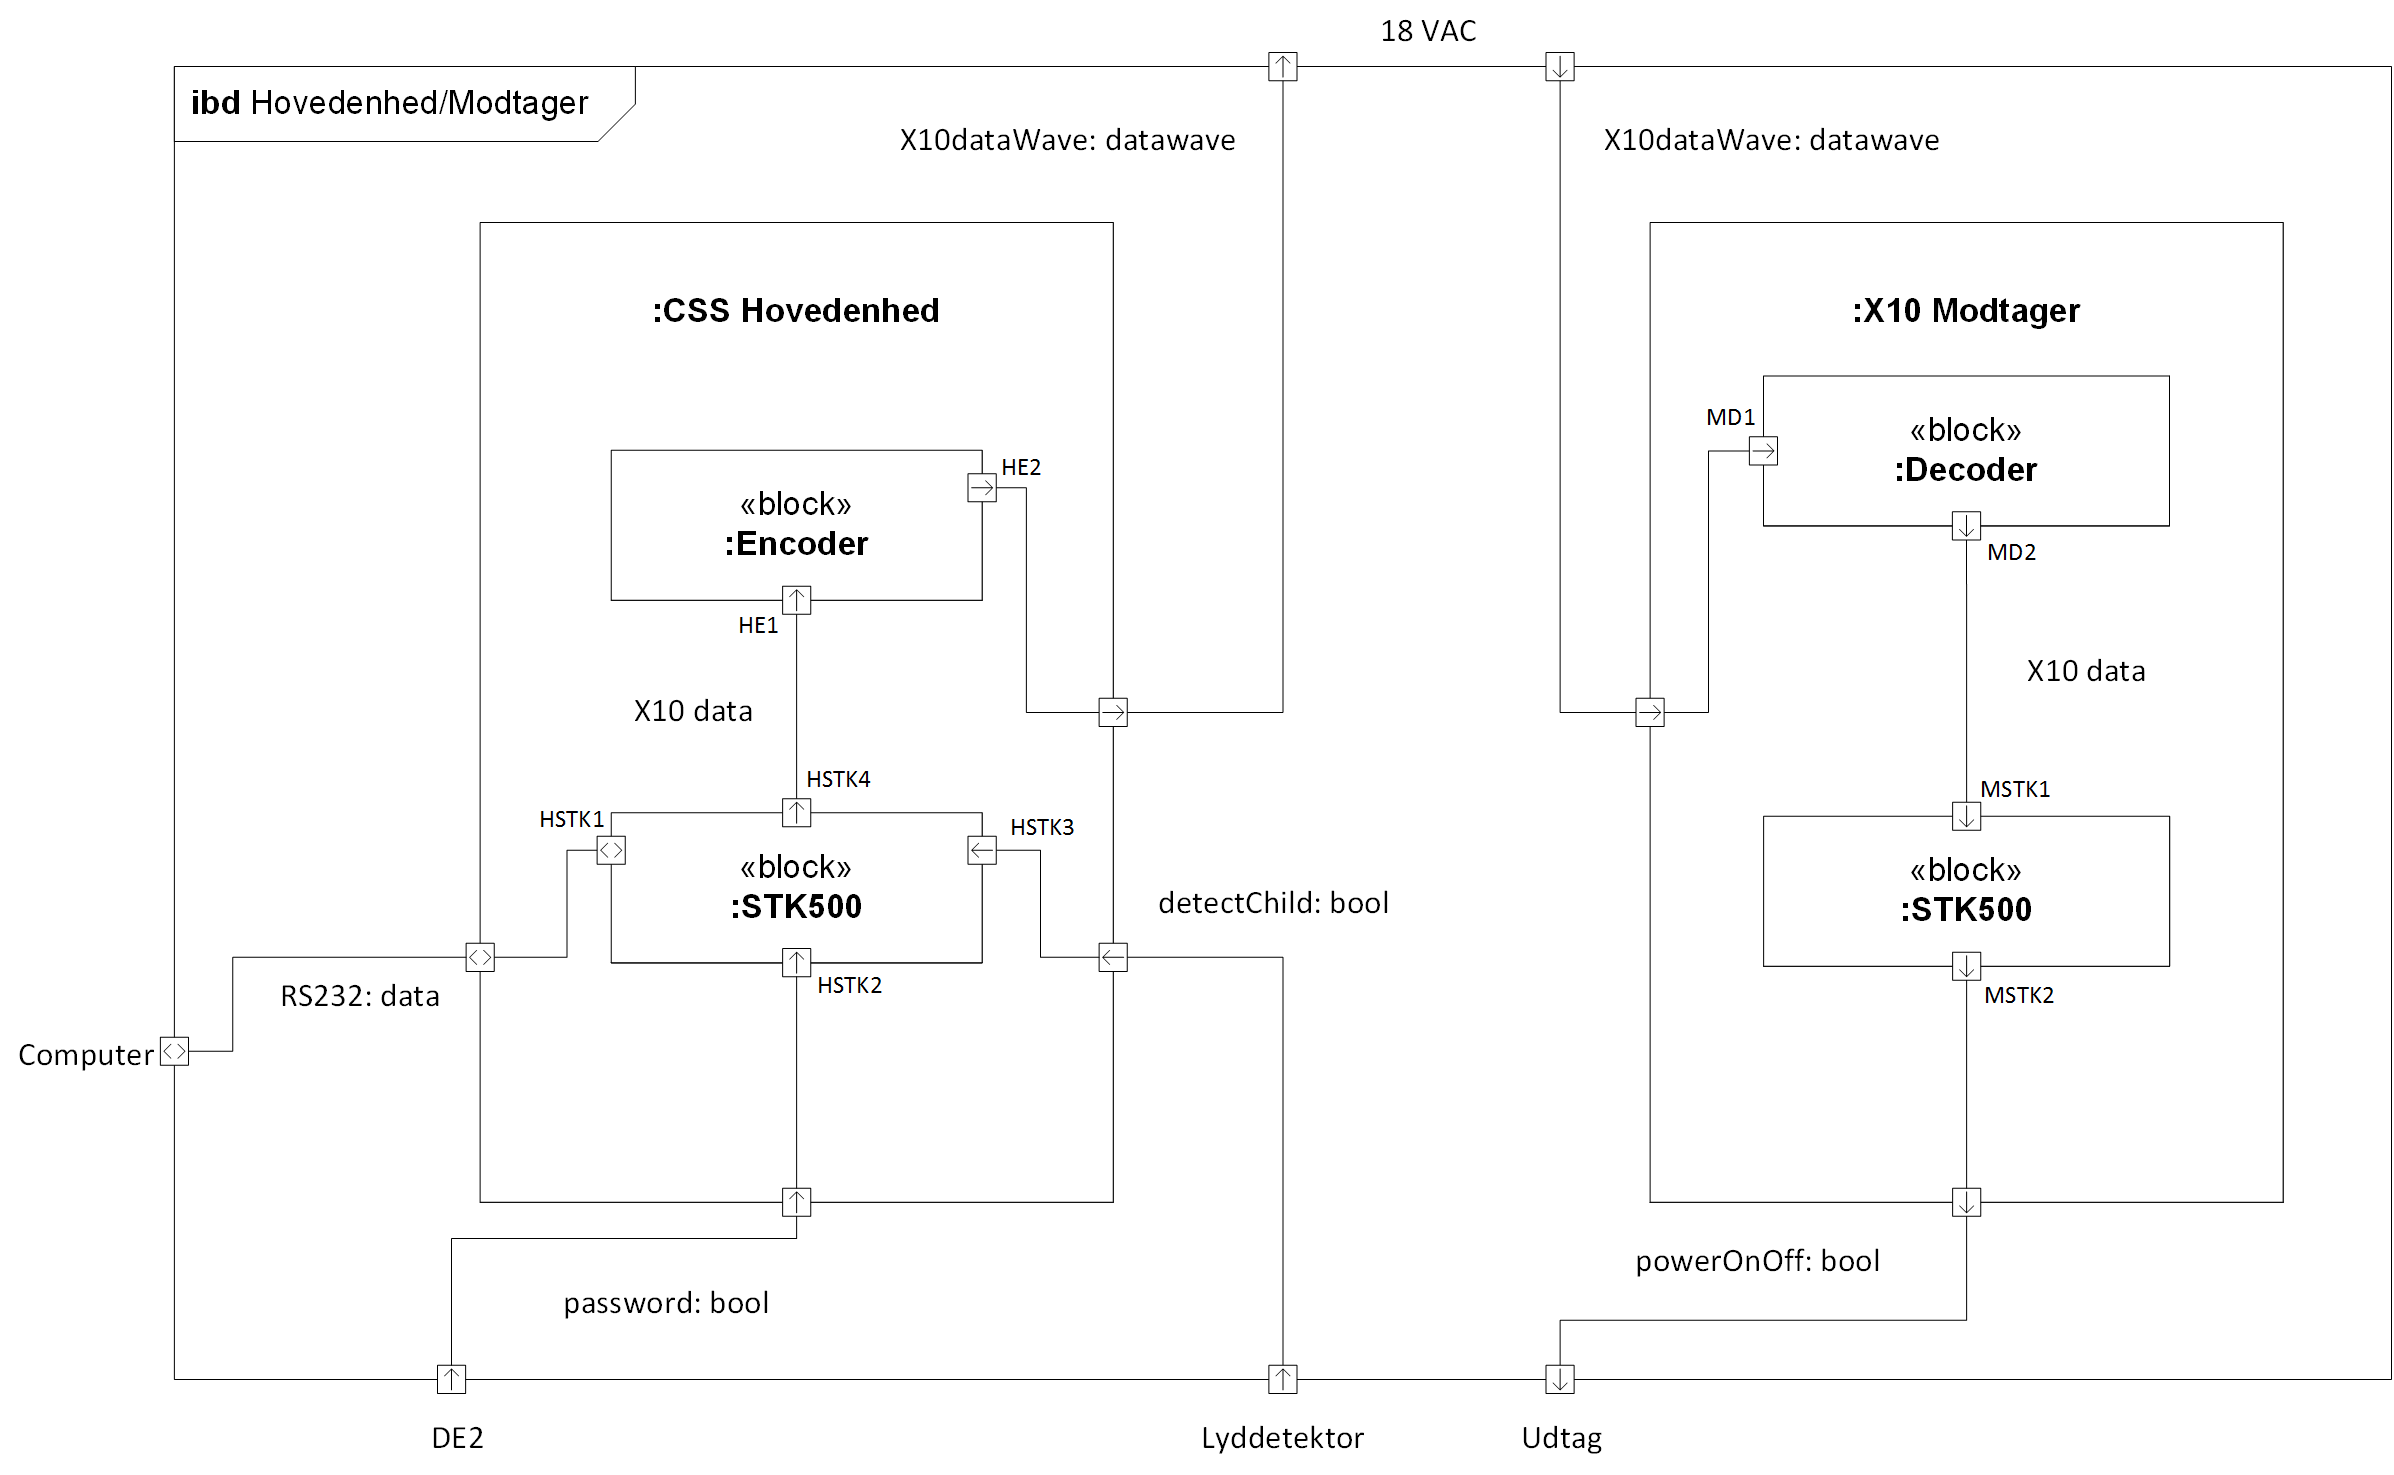
\includegraphics[width=0.9\textwidth]{billeder/diagrammer/IBD_Hovedenhed_Modtager}}
\caption{IBD CSS-hovedenhed og X10-udtag}
\label{lab:ibdhovedenhedmodtager}
\raggedright
\end{figure}
IBD diagrammet giver et internt overblik over hvordan X10-hovedenheden og X10-udtaget er forbundet. Vi ser hvilke type signaler der bliver sendt imellem de forskellige blokke.


\clearpage
\newpage

\begin{table}[htbp] %% Blok og Signal Tabel
\subsection{Grænseflade}
For at opnå forståelse for signalerne mellem blokkene laves en grænseflade der beskriver de enkelte blokkes porte og hvilke signaler der løber imellem disse.

\subsubsection{Blok beskrivelse}
Til at beskrive blokkene nærmere er anvendt tabeller som ses herunder. Her er hvert signal i en respektiv blok kommenteret og blokkens funktion er kort beskrevet. 

\caption{Tabel med beskrivelse af respektive blokke}
\begin{small}
\begin{tabular}{|p{3,3cm}|p{3,3cm}|p{3,3cm}|p{3,3cm}|}
\hline
\textbf{Bloknavn} & \textbf{Funktion} & \textbf{Signaler} & \textbf{Kommentar} \\ \hline

X10-encoder & Modtager kommandoer og encoder til 120 kHz bursts & 120 kHz & Data ud \\ \cline{3-4}	
& & X10 data & X10 data kommando ind \\ \hline

CSS-hovedenhed & Genererer X10-data og detekterer på zero-crossing & RS232 & Laptop forbindelse \\ \cline{3-4}
& & X10 data & X10 data kommando linje \\ \cline{3-4}
& & Bool & lyd detektion \\ \cline{3-4}
& & Bool & Password accept \\ \hline

X10-decoder & Modtager 120 kHz og decoder til X10 data & 120 kHz & 120 kHz ind \\ \cline{3-4}
& & X10 data & Kommando linje \\ \cline{3-4}
& & 120 kHz & 120 kHz data ind \\ \hline

X10-udtag & Modtager X10 TTL pulser og detekterer på zero-crossing & X10 data & X10 data ind \\ \cline{3-4}
&& Bool & Power I/O ekstern enhed \\ \hline 
\end{tabular}
\end{small}
\label{table:Bloktabel}
\end{table}

\begin{table}[htbp]
\subsubsection{Signal beskrivelse}
For at fuldende beskrivelsen af grænsefladen er der lavet en signaltabel som kan ses herunder. Hvert signal er beskrevet og tilknyttet en kort kommentar. Området, et signal er defineret under, er også beskrevet. Blok og terminal indgår også. 
\caption{Tabel over signaler med terminaler}
\begin{small}
\begin{tabular}{|p{2cm}|p{2cm}|p{2cm}|p{2cm}|p{2cm}|p{2,2cm}|}
\hline
\textbf{Signal-navn} & \textbf{Funktion} & \textbf{Område} & \textbf{Port 1} & \textbf{Port 2} & \textbf{Kommentar} \\ \hline

120 kHz & sende kommando på 18Vac-nettet & & Encoder, HE2 & Decoder, DM1 & \\ \hline

X10-data & kommando & & STK500, HSTK4 & Encoder, HE1 & \\ \cline{4-5}
&&& Decoder, MD2 & STK500, MSTK1 &\\ \hline

bool & digital signal & 5V/0V & DE2, N/A & STK500, HSTK2 & \\ \cline{4-5}
&&& Lyddetektor, N/A & STK500, HSTK3 & \\ \cline{4-5}
&&& STK500, MSTK2 & Udtag, N/A & \\ \hline
\end{tabular}
\end{small}
\label{table:Signaltabel}
\end{table}


